\documentclass[10pt]{article}

\usepackage{multicol}
\usepackage{array}
\usepackage{geometry}
\usepackage{longtable}
\usepackage{graphicx}
\usepackage{hyperref} 
\graphicspath{SYNCHRONY-LOGO.png}
\graphicspath{allocation.png}
\graphicspath{funding.png}
\geometry{letterpaper,tmargin=1in,bmargin=1in,lmargin=1in,rmargin=1in}

\title{%
	\textbf{Synchrony Whitepaper}\\
	\emph{On-chain Copy-Trading \& Composable Indices}}
\author{Andrew Fraser \& Andy Keh}

\begin{document}

	\maketitle
	\begin{center}
		\begin{figure}[h]
			
\includegraphics[scale=0.75]{SYNCHRONY-LOGO.png}
			\centering
		\end{figure}
	\end{center}

	\newpage
	\tableofcontents

	\newpage
		\section{Introduction}
			Over the past 18 months the blockchain industry has experienced exponential growth. The
			industry's collective market capitalization has incresaed from USD 100bn to USD 1.75tn
			(1750\%)\footnote[1]{https://www.statista.com/statistics/730876/cryptocurrency-maket-value/}.
			As a consequence of such meteoric growth, key issues surrounding the current
			implementation of blockchain technology have been placed front-and-center, chief among
			these begin scalability. 

			The largest smart-contract-enabled blockchain - Ethereum, has
			pioneered decentralised finance (Defi) and is typically the first stop for burgeoning
			ecosystem participants on their pilgrimage to Defi. However, rising transaction costs
			have created barriers to entry reminiscent of traditional finance, a new playground for
			the already wealthy, not only greatly limiting those who can participate but also
			alienating those who sought blockchain technology and cryptocurrency as the great
			equalizers. Furthermore, slow settlement cycles and low throughput have created user
			experiences vastly inferior to traditional fintech solutions and are further exacerbated
			by unintuitive and often complicated user interfaces. A combination of the
			aforementioned factors are pushing projects and users to seek better more scalable solutions.

		\subsection{The Problems}
			\subsubsection{Complexity}
					There is literally more information being created than any one user can
					sift through, filter, and digest. This sentiment is clearly reflected in
					Defi communities around the world on various forums such as the
					subreddit /r/defi, its top post being titled: ''My Brain is
					Melting``\footnote[2]{https://old.reddit.com/r/defi/comments/n802v5/my\_brain\_is\_melting/}.
					Information overload affects new users and seasoned veterans alike
					- blockchain and Defi possess a steep learning curve, from learning what
					a wallet is to implementing yield farming strategies the path to
					ecosystem fluency and a modicum of success is long and arduous - littered with
					misinformation, security vulnerabilities and scams.
					And once a participant has achieved some degree of ecosystem fluency
					they are still faced with the tremendous amount of research and
					due-diligence that is required to identify actionable signals or market
					opportunities. And while mimicking twitter trends can be profitable in
					the short-term, long-term growth and wealth building are the product of
					a more nuanced and calculated approach - optimizing portfolio
					allocations and thoroughly tested investment strategies.

					Research shows that there is a considerable cognitive overhead
					associated with context switching\footnote[3]{Meyer, D. E., Evans, J.
					E., Lauber, E. J., Gmeindl, L., Rubinstein, J., Junck, L., \& Koeppe, R.
					A. (1998). The role of dorsolateral prefrontal cortex for executive
					cognitive processes in task switching. Journal of Cognitive
					Neuroscience, 1998, Vol. 10}, a user incurs a compounding cognitive cost
					for every protocol they must interact with. A cost that is further
					exacerbated by an associated doorway
					effect\footnote[4]{https://www.scientificamerican.com/article/why-walking-through-doorway-makes-you-forget/}\footnote[5]{https://www.tandfonline.com/doi/abs/10.1080/17470218.2011.571267}:
					a psychological phenomenon where an individual forgets what they are
					doing or thinking about upon moving through a doorway. The doorway
					effect is present when switching between tabs or web-pages - each screen
					representing a metaphorical doorway a user must pass through. The
					resulting increase in tab-switching consequently leads to further
					context switches, and therefore compounds the cost of said context
					switch. Thus, from a user experience standpoint, interacting with the
					blockchain ecosystem is mentally exhausting.
				\subsubsection{Centralisation}
					With the advent of Defi, protocols seeking to emulate traditional
					investment vehicles are an inevitability. However, while claiming
					decentralisation, a lot of these protocols converge on a centralised
					oracle, and typically where it matters most. In the context of asset
					management protocols, this could be an asset manager, a council of token
					holders, or the project team. 

					Decentralised asset management is not a new concept, and has been
					explored and implemented by several other projects, a non-exhaustive
					list of these projects are:
					\begin{enumerate}
						\item Balancer;
						\item Set Protocol;
						\item Enzyme;
						\item dHedge;
						\item pieDAO; and
						\item Solrise Finance.
					\end{enumerate}
					However, all of these protocols share several glaring weaknesses, chief 
					among these being a single point of failure - they are not
					decentralised.

					All of the aforementioned protocols have a similar approach to on-chain
					asset management: pools of assets managed by an individual or an entity
					and as such, the protocol must take steps to ensure that the power
					afforded by this position cannot be abused. There are two general
					implementations of how a protocol can achieve this: the first is through
					trust-minimization, not trustlessness - performing rudimentary KYC on
					the pool's manager. Without regulation however, this is little more than
					an empty gesture; there is no means  to enforce any legal penalty for
					the misuse of a manager's power. The second is to limit how the manager
					can interact with the pool or rather, the strategies they can implement.
					For example, Bonfida created a program on the Solana blockchain named
					Bonfida Bots\footnote[6]{https://bonfida.github.io/bonfida-bot-docs/}.
					Bonfida Bots enables a user to create a pool that will execute trades
					based upon some user-defined/provided signal. Bonfida have identified
					that if the markets that a signal provider can provide signals for are
					not immutable, then the signal provider can create a mock market on the
					Serum DEX and siphon of tokens from the pool at a greatly reduced cost.
					Balancer have also identified similar weaknesses and have sought to
					''cover all their bases`` by providing private pools, where the manager
					has full control over the parameters of the pool, and public pools where,
					similar to Bonfida, the parameters are immutable and set upon
					initialisation of the pool.

					However, restriction stifles innovation - because the strategies that
					can be implemented are limited, the number of strategies will inevitably
					converge upon a small set, thus causing stagnation, and while stagnation
					is not the opposite of growth, it certainly affords the opposite of
					growth.

					The trust-minimized nature of these protocols is a symptom of the more
					serious weakness that all of these protocols bar Balancer share:
					a single point of failure. This single point of failure most commonly
					takes the form of the manager or entity managing the pool. These
					entities are under no obligation to perform their duties and certainly
					no contracts or regulation exist that can ensure or enforce performance.
					As such, a manager may even act to the detriment to the investors of
					a pool, or may be plainly negligent thus necessitating the need for the
					aforementioned approaches. More importantly however - a single point of
					failure is centralisation, meaning a lot of asset management protocols
					are incorrectly classified as Defi protocols.
					\subsection{The Solutions}
					\subsubsection{Aggregation}
					To solve the issue of a cumbersome and cognitively expensive user experience,
					a user should be able to use one application to perofrm the majority of their
					on-chain acitivies for a specific sector: i.e. an application for Defi, and an
					application for NFTs. With respect to Defi, a suser should be able to monitor
					and manage their portfolio from such an application as well as be able to
					research availble instruments or opportunities and subsequently transact upon
					them.
					\subsubsection{Customized Data}
					Performing exhaustive due diligence on every new company entering a market is
					not a viable strategy for a retail investor in traditional finance, and the same
					holds true for Defi. Investors often choose to specialize in certain types of
					opportunities and to achieve this effectively, the need to be able to tailor the
					information they receive to be relevant to those types of opportunities. Thus,
					users are interested in specific data and should therefore be able to customize
					the information the receive to be relevant to them.
					\subsubsection{Front-end Optimization}
					The goal for any front-end should be to eliminate any cost of context switching
					and to mitigate the doorway effect as much as possible. To do so, a front-end
					must have an intuitive user interface that captures a user's most logical and
					optimal workflows. Generally, a user should be able to do as much as possible
					from a dashboard, utilizing no more than four (4) ``button-presses'' without the
					interface feeling cluttered and overwhelming. Thus, each interface must have
					a clear and well-defined purpose. Effective user interface design requires
					a great deal of detail and care as well  as an intimate knowledge of potential
					users and their respective behaviours, thought processes and goals.
					\subsubsection{Indices \& Passive Investment}
					As of 2021 ETFs are a USD 8tn industry and growing at an annual rate of
					26\%\footnote[7]{https://www.bbh.com/us/en/insights/investor-services-insights/2021-global-etf-survey.html}.
					Over the past ten (10) years, 82\% of fund managers fell short of their S\&P500
					benchmark, with 94\% failing over twenty (20) years. Similarly, 73\% did not
					match up to the S\&P Midcap 400, while 76\% also underperformed the S\&P Small
					Cap
					600\footnote[8]{https://www.spglobal.com/spdji/en/documents/spiva/spiva-us-year-end-2020.pdf}.
					Active managers are consistently outperformed by indices however, there is not
					enough historical data to definitively say whether or not this holds true for
					cryptocurrencies and Defi. What is definitive is that indices are analogues for
					smart contracts - similar to how a smart contract's code can be scrutinized, so
					can an index's calculation methodology. Thus, indices are essential for
					trustless asset management and furthermore enabling a simpler, tangible, and
					quantitatively effective avenue for passive capital growth.\\
					\begin{center}
						\emph{Indices do for asset management what blockchain and smart contracts do for transactions}.
					\end{center}
					\subsubsection{Trustlessness - True Decentralisation}
					Finally, any solution must be truly trustless, truly decentralised, without
					imposing restrictive limitations upon strategy authors or asset managers while
					simultaneously ensuring the safety of its user's assets.
					\subsection{Enter Synchrony}
					Synchrony is an on-chain automated portfolio and asset management protocol
					featuring copy-trading and indices as well as wallet and protocol analytics.
					Synchrony achieves true trustlessness through the use of highly configurable
					indices that enable user to compose and index dynamic sets of tokens, liquidity
					pools, strategies and other on-chain instruments to create algorithmically
					optimized and automatically rebalancing pools or portfolios. Copy-trading
					leverages these indices enabling users to define the parameters for which
					a copy-trade is considered a candidate for execution. Synchrony's analytics and
					aggregation services enable users to make informed decisions not only with
					respect to index and copy-trade parameters but also their entire on-chain
					behaviour. To facilitate a smooth user experience, Synchrony's front-end features
					a marketplace that, along with the aforementioned suite of tools, enables users
					to interact with the entire Solana ecosystem from one location.
					\section{Core Principles}
					\subsection{Design Philosophy}
					Synchrony is built upon a modular, composable and extensible design philosophy.
					Each of Synchrony's key features are built to enhance the capabilities of the
					others while maintaining the ability to operate independently from the
					ecosystem. This philosophy extends into the resulting products - each being able
					to exist independtently or as a component of another. e.g. a copy-trade index.
					\par
					In the case of indices, each index is standalone, and an instance of any
					particular configuration of an index exists as a pool. This allows pools to be
					composed of multple indices. The one restrriction Synchron imposes upon pools is
					that they must be composed of and managed by an index. This is to ensure safety
					of the underlying assets without the need for KYC or restrictions on the
					strategies a pool initializer can implement. The modular nature of Synchrony's
					indices allow other asset management protocols to utilize them.
					\subsection{Intention-First}
					The user's intention is our top priority. A significant portion of users do not
					care if they are yield farming, staking, or liquidity mining; they care bout
					having their assets work harder for them. There is however, an obvious
					preference for instruments that are meaningful and understandable.
					\subsection{Inclusive}
					Synchrony is a platform for users of all levels of experience. Synchrony grants
					passive suers passive strategies via copy-trading and indices, active users can
					submit their wallet to be copied and featured on the Synchrony leaderboard or
					build index-pegged pools that other users can subscribe to - capitalising on the
					analytics service to drive their decisions.
					\subsection{Trustless}
					Synchrony is completely trustless, not trust-minimized. Trustless is synonymous
					with decentralised - there are no single points of failure, there are no vectors
					through which an entity can abuse its position i.e. trust is not required. \par
					Synchrony achieves this through the use of highly configurable indices; only
					the index may manage a pool or a copy-trade wallet and transact on its
					underlying assets. Each instance of an index-pegged pool is immutable; after
					a pool has been initialised its parameters cannot be changed. Indices used for
					copy-trade parameters are only mutable by the copy-trade wallet's owner.\par
					Synchrony utilizes decentralised synchronisation; anyone can execute
					protocol-critical functions as long as the conditions for execution have been
					met. For indices - rebalancing when a deviation threshold has been exceeded or
					a rebalancing interval has elapsed. For copy-trade wallets - when leader wallets
					have made valid transactions and the following wallets have pending transactions
					or settlements. \par
					Users are rewarded SCY for successfully executing these functions.
					\subsection{Non-Custodial \& Collateralised}
					Synchrony does not own any assets in any of the pools or wallets that the
					protocol manages. The user always owns their assets. Furthermore, no one
					controls the pool and no one can transact on the pool's underlying assets, only
					the program has the authority to do so, and it may only do so within the
					parameters of its index(es).
					\subsection{Fungible}
					Each index instantiated as an index-pegged pool is represented by a fungible
					token fully collateralized by its underlying tokens.
					\subsection{Dynamic}
					The Defi landscape is ever-changing, investors and ecosystem participants must
					be adaptable and be able to react swiftly to market changes. Synchrony's
					approach to copy-trading and indexing adheres to these principles. Synchrony
					enables users to define ranges or sets of instruments for both the copy-trade
					and indexing protocols to execute upon, granting dynamic allocations and
					compositions and affording granular control over strategy implementation.
					\subsection{Streamlined}
					Synchrony is built to empower all levels of users without incurring any
					unnecessary cognitive overhead. Synchrony achieves this by providing a seamless
					and intuitive interface with clearly defined and logical workflows while
					distilling information down to profile-specific signals and features by
					aggregating data and functionalities from various Defi protocols. Users only see
					the data they are interested in organized based on their preferences and needs.
					\section{Aggregation \& Analytics}
					The Synchrony analytics and aggregation services provide users detailed insights
					into the on-chain activity of wallets, tokens, products and protocols.
					\subsection{Aggregation}
					Synchrony's platform provides users a holistic view into Solana's protocols,
					enabling a user to manage their portfolio, compare assets, backtest strategies
					and transact all from a single application. Users can explore the Solana
					ecosystem filtering protocols and instruments via a range of options such as but
					not limited to:
					\begin{itemize}
						\item performance metrics with user-defined ranges (e.g. MTD, YTD, etc.):
							\begin{itemize}
								\item performance;
								\item volatility;
								\item volume;
								\item liquidity; and etc.
							\end{itemize}
						\item strategy authors;
						\item asset classes;
						\item protocols; and etc.
					\end{itemize}
					The aggregation service is a synergistic value-add to the entire Solana
					ecosystem - by providing a platform for consolidation, Synchrony enables
					user cross-pollination and generates awareness for both established and
					burgeoning protocols. Synchrony also simplifies user ecosystem experience thus spurring
					user adoption.

					\subsection{Wallet Analytics}
					Synchrony's analytics service affords users access to a granular level of detail
					regarding an ecosystem participant's on-chain behaviour. Users may simply enter
					a wallet address to retrieve data such as trade history and performance which is
					presented in a clear and easily digestible format allowing for comparisons
					against other wallets, tokens and indices. 

					Wallet analytics enable users to make
					informed decisions with respect to their own investment strategies and are also
					integral in driving leaderboard and gamification features.

					A future goal of the analytics service is to provide analytics on an
					ecosystem-wide scope granting macro-level insight into an ecosystem's
					participants' behaviours and sentiments.

					\subsection{Customization}
					Analytics can be user-configured providing a curated and tailored experience
					ensuring a user only receives data relevant to the types of opportunities they
					are interested in. 

					\subsection{Subscription-Based Service}
					The analytics service is subscription-based and charged at a monthly fee of USD
					60, payable with USDC, SOL/SCY equivalent or with a strategically partnered
					protocol's tokens at a discounted rate. All net fees are used for SCY
					repurchases. Subscriptions will eventually be tier-based - fee/trial, standard,
					pro, and enterprise - catering to users of different needs and budgets.

					\section{Copy-Trading}
					Copy-trading enables users to input a wallet address and replicate all valid
					transactions in that wallet in their own copy-trade wallet. A valid transaction
					is defined as any transaction made through another protocol, the list of which
					is governed and may be amended by the Synchrony DAO. Users can choose between
					three different methodologies for assessing whether a transaction made by
					a leader wallet is a candidate for a copy-trade:
					\begin{enumerate}
						\item Naked copy-trading - simple proportional replication of all the valid
							transactions a leader wallet executes. Naked copy-trading carries
							a significant risk associated with it - if a leader wallet is privy to
							the fact it is being followed and is owned by a malicious user, the
							leader wallet could potentially execute transactions to the disbenefit
							of the following wallets, an example would be a scenario similar to the
							Bonfida example described above. The specific use-case for naked
							copy-trading one where the user completely trusts the leader wallet
							- there is a pre-existing relationship. The protocol however does not
							restrict access to this feature - the user may use this feature at their
							own discretion and accepts the associated risks.
						\item Parameterised copy-trading - user-defined criteria for which
							a valid transaction made by a leader wallet is considered
							a candidate for a copy-trade. Parameterised copy-trading grants
							a user a relatively basic yet granular level of control over their
							copy-trade wallet's behaviour - examples of configurable parameters 
							include but are not limited to:
							\begin{itemize}
								\item frequency of replicated transactions;
								\item stop-losses;
								\item take-profits; and
								\item whitelisted tokens/protocols.
							\end{itemize}
						\item Index-driven copy-trading - dynamic whitelisting of candidate tokens,
							protocols or instruments. Index-driven copy-trading builds upon
							parameterised copy-trading by utilizing indices to define when a valid
							transaction made by a leader wallet is considered a candidate for
							a copy-trade. For example, copy-trade wallets utilizing the Solana
							Ecosystem Index will only replicate transactions on tokens that are
							present in that index. The default setting for index-driven copy-trading
							utilizes a combination of Synchrony composed indices however, users may
							choose to utilize any index or combination of indices on the Synchrony
							platform as well as construct their own.
					\end{enumerate}

					\subsection{Leveraging the Ledger}
					Blockchains are transparent and immutable ledgers, anyone can peruse the record
					of transactions made by any participant on the network. This is a powerful tool
					for not only analytics but also for copy-trading. In off-chain implementations
					of copy-trading only traders who are approved by the platform and opt-in to
					having their trades copied can be copy-traded, and thus, any data and analytics
					available to a user regarding copy-trading is limited to that scope. On-chain
					however, there are no such limitations - a wallet does not need to be listed on
					the Synchrony marketplace in order for a user to be able to see the
					transactions it is executing, and therefore, a wallet does not need to be listed
					on the Synchrony marketplace for a user to be able to copy-trade it. Synchrony
					still remunerates unlisted wallets however, there are advantages for a wallet to
					be listed on the Synchrony marketplace, some of which are described below.

					\subsection{Subscription-Based Service}
					Copy-trading is a subscription-based service and charged at a monthly fee of USD
					30, payable with USDC, SOL/SCY equivalent or with a strategically partnered
					protocol's tokens at a discounted rate. Leader wallets that are listed on the
					Synchrony marketplace are remunerated \(\frac{2}{5}\) or USD 12 of the
					subscription fee
					for each wallet that is following it, Synchrony receives \(\frac{2}{5}\) or USD 12 as
					a platform fee and \(\frac{1}{5}\) or USD 6 is granted proportionally to users who stake SCY
					on that wallet. Wallets that are not listed on the marketplace will be
					remunerated at USD 6 per month, with the rest of the fee granted to Synchrony.
					The subscription fee is antecedently charged monthly to followers and
					distributed at the end of the month to stakeholders.

					\subsection{Leaderboard}
					Wallets listed on the Synchrony marketplace are eligible to be featured on the
					copy-trade leaderboard. Consistently profitable wallets can garner community
					accolades and privileges including but not limited to cosmetics that showcase
					their standing. The leaderboard will be the focal point of competitions and
					time-based events that will drive community engagement and contribution.
					Furthermore, maintaining a position on the leaderboard grants users a SCY reward
					proportional to their average 7d performance and enters them into
					a community-driven lottery.

					\section{Indexing}
					Synchrony's indices have three general implementations and an unlimited number
					of configurations. The three (3) general implementations are:
					\begin{enumerate}
						\item Synchrony composed indices - indices composed by the team in
							conjunction with our strategic partners. The aim of Synchrony composed
							indices is to provide consumers anm entrypoint and/or passive investment
							strategy with a focus on the assets and instruments present on the
							Solana ecosystem. These indices may be created and governed by the
							Synchrony DAO.
						\item Community composed indices - these indices are composed by the
							community, there are not restrictions on these indices besides the
							static fee set by the Synchrony DAO which is uniform across all indices,
							and that there may only be one particular instance of a specific
							configuration of an index.
						\item Portfolio-level indices - these indices are implemented at a portfolio
							level and are typically utilized for automated portfolio management,
							these indices are not visible to the community unless permitted by the
							author. Portfolio-level indices have no associated token.
					\end{enumerate}

					\subsection{Configurable}
					Each of Synchrony's indices are completely configurable, affording investment
					strategies with a high degree of specificity. A user can define the parameters
					for which an asset or strategy would be considered a candidate for inclusion
					into a pool - essentially delineating a dataset. The index can then be
					configured with:
					\begin{itemize}
						\item chosen weighting metric; 
						\item minimum and maximum weights;
						\item rebalancing period; 
						\item deviation threshold; 
						\item the minimum and naximum number of assets to be returned by the index;
							and etc.
					\end{itemize}
					\subsubsection{Whitelisting}
					Whitelisting enables users to specify tokens or instruments for a dataset they
					want an index to evaluate. For example, a user may wish to evaluate only
					specific tokens on the Solana Ecosystem Index instead of the entire index and
					weigh them accordingly. Whitelisting is the feature that enables a high degree
					of specificity - enabling strategy authors a large degree of freedom with
					respect to strategy implementation without imposing overly restrictive
					limitations.

					\subsection{Dynamic}
					Most on-chain implementations of an index exist as static weights and static
					compositions where rebalancing returns a pool to its initial state. No on-chain
					implementations of an index-pegged pool implement dynamic compositions. For
					exmaple, when DPI by Index Coop makes a change to the pool's composition it
					undergoes a complete reconstitution, a limitation imposed upon the pool by Set
					Protocol's design. Synchrony is different, not only are the weights dynamically
					adjusted to track a proper implementation of an index, the pool's composition is
					also dynamic as the protocol has the authority to add and remove assets from the
					pool.

					\subsection{Composable \& Modular}
					Each index is instantiated as an index-pegged pool with an accompanying fungible
					token representing proportional ownership of its underlying assets. Indices can
					therefore compose, or be composed of another index's tokens.

					\subsection{Powerful}
					Synchrony's indices are suitable for a wide range of use-cases, from portfolio
					management to copy-trading. One of the more powerful features of Synchrony's
					indices, alongside their configurability, is the ability to index any on-chain
					instrument. From tokens, to liquidity pools, to strategies and even indices
					themselves, there is very little that Synchrony's suite of indices cannot
					evaluate. Where Synchrony does not have coverage, Synchrony will rely on the
					strength of its community and DAO.
					
					\subsection{Mechanics}
					Indices generate revenue via an immutable transaction fee of 0.25\%. Transaction
					fees are charged upon the construction and deconstruction of index-pegged pool
					tokens.
					To construct a pool token, the user must provide the underlying assets in their
					relevant weights however, the protocol is capable of performing transitive swaps
					on the Serum DEX enabling a single-asset entry/exit.

					\subsubsection{Synchrony-Composed Index Mechanics}
					Synchrony composed indices possess the same immutable fees as any other index
					however, only approved providers - users who stake an amount of SCY as
					determined by the Synchrony DAO, are able to construct and deconstruct pool
					tokens.
					Synchrony will mainting liquidity pools for each Synchrony-composed index's
					pool token - e.g. ETF/SOL. Synchrony incentivizes approved providers to
					capitalise on the arbitrage opportunity created by these swap pools and not any
					other third-party liquidity pools by waiving the transaction fee for the construction and deconstruction of pool tokens
					if the token is immediately swapped into one of the corresponding liquidity
					pools. This is achieved via executing the instruction:
					\begin{verbatim}PoolInstruction::TokenEvent(EventType::Arbitrage(NonZeroU64))\end{verbatim} 
					itself executing:
					\begin{verbatim}PoolInstruction::TokenEvent(EventType::Create(NonZeroU64))\end{verbatim} and
					subsequently: \begin{verbatim}SwapInstruction::Swap(NonZeroU64)\end{verbatim} in one transaction.

					\section{Synchrony Indices}
					\subsection{The Solana Ecosystem Index (SEI)}
					The Solana Ecosystem Index tracks the top tokens on the Solana Ecosystem with
					a market capitalization of over USD 10mm. This index is weighted by market cap
					and is capped at thirty-two (32) tokens. Each token has a maximum weight of
					30\%, there is no minimum token weighting upon initialisation. This index has
					a rebalancing interval of twenty-four (24) hours which elapses at 0000 UTC daily
					and has a deviation threshold of 20\% where a token's market cap must deviate
					20\% from it's previous market cap before a pre-interval rebalance may be
					triggered. A manual rebalance may be performed by approved providers by providing the underlying assets in
					weights that may resolve the delta. Manual rebalances are subject to a grace
					period - after such period has elapsed, any user
					may permissionlessly trigger an automatic rebalance with the necessary
					transactions being executed on Serum DEX at spot
					prices.

					This index utilizes an adjustment methodology based on the Paasche formula:
					\[I^{pass}_t = I^{pass}_{t-1}\frac{\sum_{i=1}^n P_{i,t}Q_{i,t}}{\sum_{i=1}^n
					P_{i,t-1}Q_{i,t}}\]

					The following parameters may be altered by a vote of simple majority made by the
					Synchrony DAO:
					\begin{itemize}
						\item number of tokens permitted in the index;
						\item minimum market cap;
						\item minimum token weight;
						\item maximum token weight;
						\item rebalancing period; and
						\item deviation threshold.
					\end{itemize}

					\subsection{The Raydium Liquidity Pool Index (RAI)}
					The Raydium Liquidity Pool index tracks the highest yielding liquidity pools on
					the Raydium protocol with a minimum liquidity requirement of USD 1mm. Tokens in
					candidate liquidity pools must be composed of one stable coin OR possess
					correlative volatility. This index
					is weighted by volume and is capped at eight (8) tokens. Each token has a maximum
					weight of 30\%, there is no minimum token weighting upon initialisation. This
					index has a rebalancing interval of twenty-four (24) hours which elapses at 0000
					UTC daily and has a deviation threshold of 20\% where a liquidity pool's
					liquidity must deviate 20\% from its previous liquidity before a pre-interval
					rebalance may be triggered. The following parameters may be alter by a vote of
					simple majority made by the Synchrony DAO:
					\begin{itemize}
						\item weighting parameter;
						\item number of tokens permitted in the index;
						\item minimum pool liquidity;
						\item minimum token weight;
						\item maximum token weight;
						\item rebalancing threshold; and
						\item deviation threshold.
					\end{itemize}

					\subsection{The Stable Coin Index (STX)}
					The Stable Coin Index tracks all stable coins on the Solana ecosystem (at the
					time of writing USDC \& USDT) and weights them equally. This index is rebalanced
					daily at 0000 UTC.

					The parameters of this index may not be altered by DAO vote.

					\subsection{The Synchrony Composite Index}
					The Synchrony Composite Index is a value-weighted index composed of the Solana
					Ecosystem Index and the Raydium Liquidity Pool Index weighted 70/30 respectively
					with the aim of emulating a traditional portfolio allocation. This index has
					a rebalancing interval of seven (7) days which elapses at 0000 UTC every Sunday
					and a deviation threshold of 15\% where on of the underlying components' value
					must deviate 15\% from its previous rebalance value before a pre-interval
					rebalance can be triggered. The following parameters may be altered by a vote
					of simple majority made by the Synchrony DAO:
					\begin{itemize}
						\item weighting parameter;
						\item number of tokens permitted in the index;
						\item minimum market liquidity;
						\item minimum token weight;
						\item maximum token weight;
						\item rebalancing period; and
						\item deviation threshold.
					\end{itemize}

					While the underlying composition may be subject to alteration via DAO vote, the
					Solana Ecosystem Index will always compose a minimum of 30\% of the index.

					\section{The Synchrony Token}
					SCY is the native token of the Synchrony platform, providing an asset the holder
					can use for staking rewards, unlocking premium features, yield farming, and
					discounts. It will grow in value based on the revenue generated by the Synchrony
					platform.
					\begin{itemize}
						\item All net platform fees go towards the Synchrony token;
						\item users staking SCY receive a discount for platform services;
						\item SCY may be used to pay fees across the platform;
						\item SCY holders may use SCY to purchase premium features such as ``banner
							space''\footnote[8]{``Banner space'' is ``real-estate'' on the
							marketplace where a wallet or index-pegged pool may be featured.} and
							profile customisation options;
						\item SCY will be rewarded for staking and
							synchronisation\footnote[9]{Synchronisation is defined as interacting
							with the protocol in order to execute protocol-critical functions, this
							includes but is not limited to rebalancing.};
						\item SCY holders may stake SCY on wallets or indices as a form of
							``insurance''/``validation'', this grants the staker a share of the fees
							generated by the wallet/index\footnote[10]{If the staked-on instrument
							consistently performs poorly, a portion of the staked tokens are
							forfeited to the users subscribed to the instrument};
						\item SCY holders may participate in limited governance of the Synchrony
							platform; and
						\item data for indices is provided by ecosystem participants voted on by the
							Synchrony DAO. Data providers must meet a minimum capital requirement,
							decided on by the DAO, of staked SCY tokens. These tokens go towards
							a platform insurance pool. Providers are granted an equal share of all
							fees generated by Synchrony composed indices.
						\item index token construction and deconstruction may only be performed by
							approved providers. Any platform participant may become an approved provider by
							staking a certain amount of SCY the exact amount being decided by the
							Synchrony DAO.
					\end{itemize}

					\section{Governance}
					SCY holders can submit proposals for changes and improvements to Synchrony. Some
					examplesexamples  of proposals are:
					\begin{itemize}
						\item implementation priority of integrations with other protocols;
						\item utility features for the SCY token; and
						\item parameter adjustment for certain Synchrony composed indices.
					\end{itemize}

					Initially proposals will need to be approved by the project team \& advisors.
					They will help guide the proposal and evaluation process for up to thirty-six
					(36) motnhs to allow for the community and platform to be built out and ensure
					significant participation from SCY holders.

					In order to propose a topic for voting, users will need to pay a deposit of SCY.
					If the proposal receives a simple majority (51\%) of the votes the proposer
					will receive their entire SCY deposit back.

					A minimum threshold for the required number of votes must be met for each stage
					a proposal goes through in order for a proposal to pass.

					The process for voting is as follows:
					\begin{enumerate}
						\item one (1) week for proposals; and
						\item one (1) week for voting on proposals
					\end{enumerate}

					\section{Roadmap}
					\subsection{Phase 0 - Protocol Demo}
					The Synchrony protocol demo will be streamed live on September 14th 2021, the
					demo will feature basic copy-trading functionality and the release of the Solana
					Ecosystem Index onto the Solana Devnet for testing. The front-end will feature
					integrations with Serum, Raydium and Orca enabling users to perform swaps
					utilising all three (3) protocols as well as provide liquidity to Raydium \&
					Orca directly from the Synchrony dashboard. The aforementioned features will be
					made available to users in a selective closed-beta.

					\subsection{Phase I - Solana Devnet Launch}
					Phase I will feature Mainnet launch of all Synchrony composed indices:
					\begin{enumerate}
						\item the Solana Ecosystem Index;
						\item the Raydium Liquidity Pool Index;
						\item the Stable Coin Index; and
						\item the Synchrony Composite Index.
					\end{enumerate}
					Copy-trading and automated portfolio management via static indices will be
					available for open-beta testing on Devnet. Backtesting and limited analytics
					will be available on Mainnet with additional features on a rolling release
					schedule.

					\subsection{Phase II - Solana Mainnet Launch \& TGE}
					Mainnet launch of Copy-trading featuring integrations with Mango Markets, Serum
					\& Raydium will coincide with Synchrony's token generation event. The target
					date for Mainnet launch is early January 2022.

					\subsection{Phase III - Mainnet Launch of Composable Indices \& Feature Expansion}
					Mainnet launch of composable indices marks the full release of version 1.0 of
					the Synchrony platform. Phase III will also explore the development of social
					analytics features such as platform trends, social searching and news
					aggregation.

					\subsection{Phase IV \& Beyond - Cross-Chain Integration}
					Phase IV will ramp up tooling for cross-chain integration with an expected
					rolling release model of six (6) weeks development followed by six (6) weeks of
					testing, culminating in a Mainnet launch by the end of each quarter.

					\section{Tokenomics}
					Token Symbol: SCY\\
					Total Token Supply: 1,000,000,000.00\\
					Token Allocation by Percentage:

					\begin{center}
						\begin{figure}[h]
							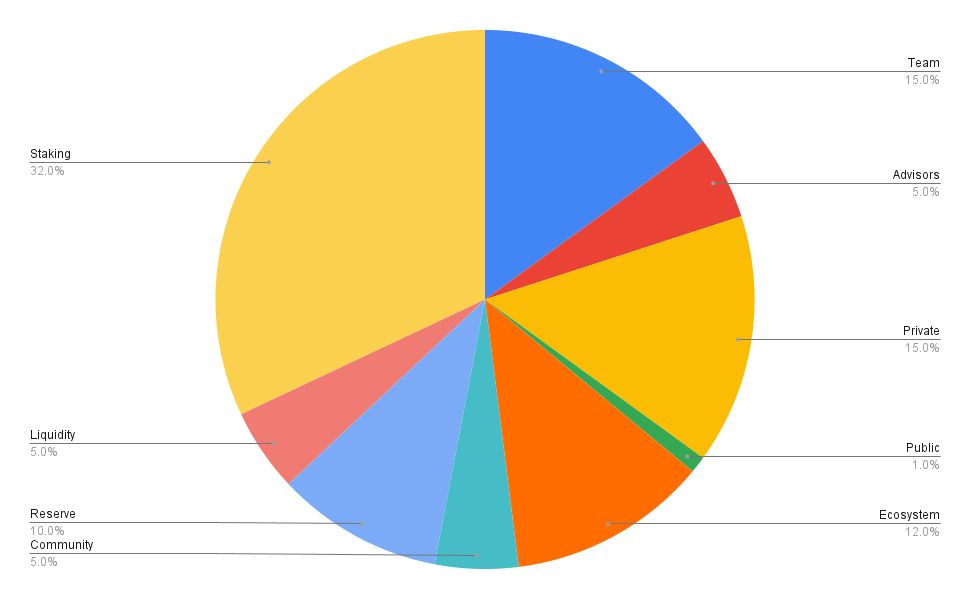
\includegraphics[scale=0.5]{allocation.png}
							\centering
						\end{figure}
					\end{center}

					\subsection{Team}
					The Synchrony team will be vested on a thirty-six (36) month timeline, 1/24 of
					team tokens will be emitted on the one (1) year anniversary of the Token
					Generation Event and every month thereafter. 15\% of the total token supply is allocated
					to the Synchrony team.

					\subsection{Advisors}
					Synchrony advisors will be vested on the same schedule as the team. 5\% of the
					total supply is allocated for advisors.

					\subsection{Private}
					\subsubsection{Round 1}
					Round 1 tokens are vested on a fifteen (15) month timeline, 5\% of which are
					emitted on the date of the Token Generation Event. 1/15 of the remaining vested
					tokens are emitted each month thereafter on the same day of the month as the
					Token Generation Event. 3\% of the total token supply is allocated to Round
					1 investors, token price is set at USD 0.02.

					\subsubsection{Round 2}
					Round 2 tokens are vested on a twelve (12) month timeline, 10\% of which are
					emitted on the date of the Token Generation Event. 1/12 of the remaining vested
					tokens are emitted each month thereafter on the same day of the month as the
					Token Generation Event.
					monthly emissions on the same day as the Token Generation Event. 12\% of the total
					token supply is allocated to Round 2 investors, token price is set at USD 0.03.

					\subsection{Public}
					Public sale tokens will follow no vesting period and participants of the public
					sale will therefore receive
					100\% of their tokens. 1\% of total token supply is allocated for the public sale,
					token price is set at USD 0.06.

					\subsection{Ecosystem}
					Ecosystem token allocation is to ensure and encourage a vibrant community.
					Ecosystem token allocation is specifically used to support partnerships,
					grants and development programs. 12\% of the total token
					supply is allocated for ecosystem growth. Ecosystem tokens are vested for
					twenty-four (24) months with monthly emissiosn. The longer time horizon
					was chosen to ensure that growth remains constant allowing Synchrony and its
					community to mature and foster innovative and meaningful partnerships.

					\subsection{Liquidity}
					Liquidity token allocation primarily serves the function of maintaining
					liquidity on exchange listings. 5\% of the total token supply is allocated for
					liquidity without any vesting period.

					\subsection{Community}
					Community token allocation is for user acquisition, engagement and management.
					5\% of the total token supply is allocated for community growth. Community
					tokens are vested over a twenty-four (24) month period with monthly emissions.

					\subsection{Reserve}
					Reserve allocation may be utilised in any of the aforementioned areas for which
					there may be a shortfall due to unforeseen circumstances or increased demand.
					Reserve allocation may also be used for any further raise Synchrony requires
					specific to cross-chain integrations. 5\% of the total token supply is allocated
					for reserve vested over a twelve (12) month period with monthly emissions.

					\subsection{Staking}
					Synchrony's protocol accounts for staking with an initially inflationary model
					with a decreasing rate until a terminal floor is reached. This is necessary for
					rapid initial growth of the protocol and to bootstrap liquidity. 32\% of the
					total token supply is allocated for staking vested over a twelve (12) month
					period with monthly emissions.

					\section{Funding Allocation}
					Total Raise: USD 4,200,000.00\\
					Funding Allocation by Percentage:

					\begin{center}
						\begin{figure}[h]
							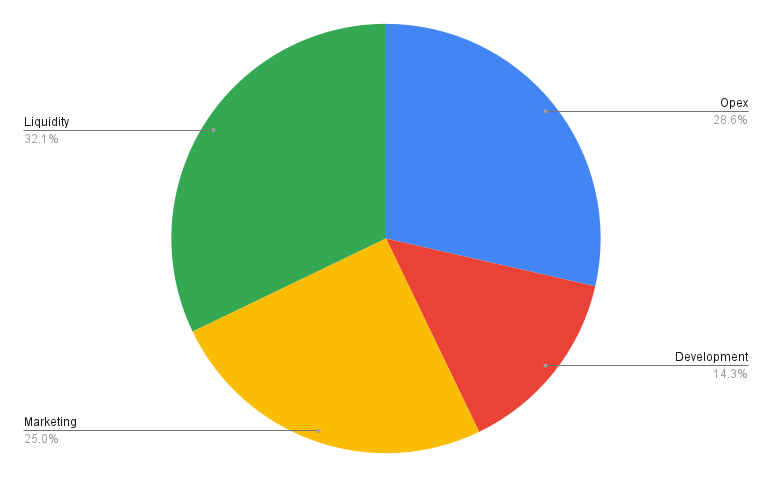
\includegraphics[scale=0.6]{funding.png}
							\centering
						\end{figure}
					\end{center}

					\section{Solana}
					We built Synchrony on Solana as we believe Solana is the next generation
					blockchain. It is the objective winner in terms of scalability, currently able
					to process over 65,000 transactions per second with a settlement cycle of 400ms.
					This is forecast to scale with Moore's law of parallelism to a maximum
					theorhetical throughput of 700,000 transactions per second and 150ms.

					Frequently rebalancing indices and copy-trades necessitate not only a blockchain
					with a high throughput and fast settlement cycle, but also one with negligible
					transaction costs - transaction costs on Ethereum are value destroying.

					Furthermore, only Solana possesses all the traits necessary to provide user
					experinces that are on-par with current fintech solutions.

					\section{The Synchrony Team}
					The Synchrony team (Synchrony Labs) is an international team of engineering and
					finance professionals with a single shared goal - to build blockchain
					technologies that are useful, lasting and high quality.

					Each member brings decades of experience in their respective fields: asset
					management, fintech, software development, blockchain and entrepreneurship.

					We built this platform for ourselves as much as anybody else, addressing
					significant shortcomings across all blockchains and traditional asset management
					sectors.
					\vspace{1em}

					\noindent The Synchrony team is lead by:
					\subsection{Andrew Fraser} - a software engineer with a decade of experience designing and
					developing solutions for tier-1 financial institutions with a speciality in
					execution platforms, algorithmic trading and algorithmic portfolio optimization.
					He was a former director of Prive technologies, a Hong Kong based fintech
					start-up, their execution platform Avenir / Wealth and i-Invest: an in-house
					execution platform for Ageas Insurance Company Asia (AICA).
					\subsection{Andy Keh} - a serial entrepreneur with over a decade of experience in application
					and systems development. He is a former operations manager at the digital
					marketing agency c-4 analytics, director of the R\&D division for a Berkshire
					Hathaway subsidiary H.H. Brown, and the founder of a alternative asset
					management and digital marketing company - Sentience.

					\section{Contact}
					Official Website: https://synchrony.fi\\
					Twitter: @SynchronyFi\\
					Email: contact@synchrony.fi


					

	\end{document}
